\section{REINFORCE}
\begin{frame}{}
    \LARGE Reinforcement Learning: \textbf{REINFORCE}
\end{frame}

\begin{frame}{REINFORCE}
\begin{itemize}
    \setlength{\itemsep}{1em}
    \item REINFORCE is an elegant algorithm for maximizing the expected return.
    \item Intuition: trial and error.
    \item Sample a trajectory $\tau$. If you get a high reward, try to make it more likely; if you get a low reward, try to make it less likely.
    \item A trajectory is a sequence of states, actions, and rewards: $\tau = (s_0, a_0, r_0, s_1, a_1, \cdots)$.
\end{itemize}
\end{frame}

% ---------------------------------------------------------------------------
% 1. The objective
% ---------------------------------------------------------------------------
\begin{frame}{REINFORCE: The Objective}
Our objective is the \textbf{expected} discounted return, where $r(\tau) := \sum_{t \geq 0} \gamma^t r_t$ is the return of one trajectory:
$$\mathcal{J}(\theta) = \mathbb{E}_{\tau \sim p(\tau;\theta)}\left[ r(\tau) \right] = \int_\tau r(\tau)\, p(\tau;\theta)\, d\tau$$

\only<1>{%
\begin{block}{Reminder: an expectation is a probability-weighted average}
$\displaystyle \mathbb{E}_{x \sim p}[f(x)] = \sum_x \underbrace{p(x)}_{\text{how likely}}\,\underbrace{f(x)}_{\text{value}}$ \;\; (or $\int p(x)f(x)\,dx$ if continuous).
Here each ``outcome'' is a whole trajectory $\tau$: its value is $r(\tau)$ and its weight is how likely the policy is to produce it.
\end{block}}

\only<2->{%
Differentiate w.r.t.\ $\theta$. The gradient moves inside the integral, and $r(\tau)$ carries no $\theta$ (the rewards of a \emph{fixed} trajectory don't change with the weights), so only $p(\tau;\theta)$ is differentiated:
$$\nabla_\theta \mathcal{J}(\theta) = \int_\tau r(\tau)\, \nabla_\theta p(\tau;\theta)\, d\tau$$
where the probability of a trajectory factorises as
$$p(\tau;\theta) = \underbrace{p(s_0)}_{\text{start state (no }\theta\text{)}} \prod_{t \geq 0} \underbrace{p(s_{t+1}|s_t, a_t)}_{\text{environment (no }\theta\text{)}}\, \underbrace{\pi_\theta(a_t|s_t)}_{\text{our policy}}$$}
\end{frame}

% ---------------------------------------------------------------------------
% 2. Why this is intractable: two problems
% ---------------------------------------------------------------------------
\begin{frame}{REINFORCE: Why We Can't Use This Directly}
This gradient is \textbf{intractable} --- for two distinct reasons that the rest of the derivation will fix one at a time.
\vspace{0.4em}
\begin{block}{Problem 1 --- we have no way to actually compute this}
The integral runs over \emph{every possible trajectory} --- far too many to add up directly. Our only tool for such a sum is \textbf{Monte Carlo}: run the policy and average what happens. But that works only when each trajectory is weighted by a genuine probability $p(\tau;\theta)$ (non-negative, sums to $1$) --- then ``sampling'' means playing episodes. Here the weight is $\nabla_\theta p(\tau;\theta)$, a \emph{change} in probability, not a probability: it can be negative and it sums to $0$. You cannot play an episode to ``sample'' a change, so Monte Carlo does not apply.
\end{block}
\pause
\begin{block}{Problem 2 --- it needs a model of the environment}
$p(\tau;\theta)$ contains $p(s_0)$ and $p(s_{t+1}|s_t, a_t)$: the environment's dynamics, which we \textbf{do not know} and cannot differentiate.
\end{block}
\end{frame}

% ---------------------------------------------------------------------------
% 3. Fix Problem 1: the log-derivative trick
% ---------------------------------------------------------------------------
\begin{frame}{REINFORCE: Fixing Problem 1 --- Back to an Expectation}
\textbf{Goal:} rewrite the gradient as an expectation $\mathbb{E}_{\tau \sim p(\tau;\theta)}[\,\cdots]$ --- the \emph{only} form we can estimate, by rolling out the policy and averaging.
\pause
\vspace{0.5em}

\textbf{The log-derivative trick} --- multiply and divide by $p(\tau;\theta)$:
$$\nabla_\theta p(\tau;\theta) = p(\tau;\theta)\, \frac{\nabla_\theta p(\tau;\theta)}{p(\tau;\theta)} = p(\tau;\theta)\, \nabla_\theta \log p(\tau;\theta)$$
This manufactures a factor of $p(\tau;\theta)$ --- exactly the sampling weight an expectation needs.
\pause
\vspace{0.3em}

Substitute it back into $\nabla_\theta \mathcal{J}$:
$$\nabla_\theta \mathcal{J}(\theta) = \int_\tau \big( r(\tau)\, \nabla_\theta \log p(\tau;\theta) \big)\, p(\tau;\theta)\, d\tau = \mathbb{E}_{\tau \sim p(\tau;\theta)}\!\left[ r(\tau)\, \nabla_\theta \log p(\tau;\theta) \right]$$
It \emph{is} an expectation now $\Rightarrow$ estimate it by Monte Carlo. \textbf{Problem 1 solved} (Problem 2 still hides inside $\log p$).
\end{frame}

% ---------------------------------------------------------------------------
% 4. Fix Problem 2: the dynamics drop out
% ---------------------------------------------------------------------------
\begin{frame}{REINFORCE: Fixing Problem 2 --- The Dynamics Drop Out}
\textbf{Goal:} the log-probability $\log p(\tau;\theta)$ still contains the unknown environment terms. Watch them vanish under $\nabla_\theta$.
\vspace{0.2em}

Recall the trajectory probability is a \textbf{product} over timesteps:
$$p(\tau;\theta) = p(s_0) \prod_{t \geq 0} p(s_{t+1}|s_t, a_t)\, \pi_\theta(a_t|s_t)$$
\pause
Taking $\log$ turns this product into a \textbf{sum} (and since $\log$ is increasing, maximizing $\log p$ is the same as maximizing $p$):
$$\log p(\tau;\theta) = \log p(s_0) + \sum_{t \geq 0} \Big[ \log p(s_{t+1}|s_t, a_t) + \log \pi_\theta(a_t|s_t) \Big]$$
\pause
Differentiate. Every term without $\theta$ becomes zero --- the start state $\log p(s_0)$ and \emph{all} dynamics $\log p(s_{t+1}|s_t, a_t)$:
$$\nabla_\theta \log p(\tau;\theta) = \sum_{t \geq 0} \nabla_\theta \log \pi_\theta(a_t|s_t)$$
\pause
Only our own policy survives $\Rightarrow$ the estimator is \textbf{model-free}. \textbf{Problem 2 solved.}
\end{frame}

% ---------------------------------------------------------------------------
% 5. The estimator
% ---------------------------------------------------------------------------
\begin{frame}{REINFORCE: The Gradient Estimator}
Put both fixes together: start from the expectation (Problem 1 fix) and substitute $\nabla_\theta \log p = \sum_{t \geq 0} \nabla_\theta \log \pi_\theta(a_t|s_t)$ (Problem 2 fix):
\begin{equation*}
\begin{split}
    \nabla_\theta \mathcal{J}(\theta)
    & = \mathbb{E}_{\tau}\!\left[ r(\tau)\, \nabla_\theta \log p(\tau;\theta) \right] \\
    & = \mathbb{E}_{\tau}\!\left[ r(\tau) \sum_{t \geq 0} \nabla_\theta \log \pi_\theta(a_t|s_t) \right]
      \approx \sum_{t \geq 0} r(\tau)\, \nabla_\theta \log \pi_\theta(a_t|s_t)
\end{split}
\end{equation*}
{\footnotesize (Last step: one sampled trajectory $\tau$. Here $r(\tau)$ is constant over $t$, so it could equally sit outside the sum --- we keep it inside because the next section replaces it with a \emph{per-timestep} weight.)}
\pause
\vspace{0.2em}

\textbf{Interpretation:} $\nabla_\theta \log \pi_\theta(a_t|s_t)$ points in the direction that makes $a_t$ \emph{more likely}; the scalar $r(\tau)$ signs and scales that push:
\begin{itemize}
    \item $r(\tau)$ high $\Rightarrow$ increase the probability of the actions taken;
    \item $r(\tau)$ low / negative $\Rightarrow$ decrease them.
\end{itemize}
\pause
Crediting every action with the \emph{whole}-trajectory return looks crude --- but it is \textbf{unbiased}: in expectation, it averages out.
\end{frame}

\begin{frame}{REINFORCE}
    \begin{figure}
        \centering
        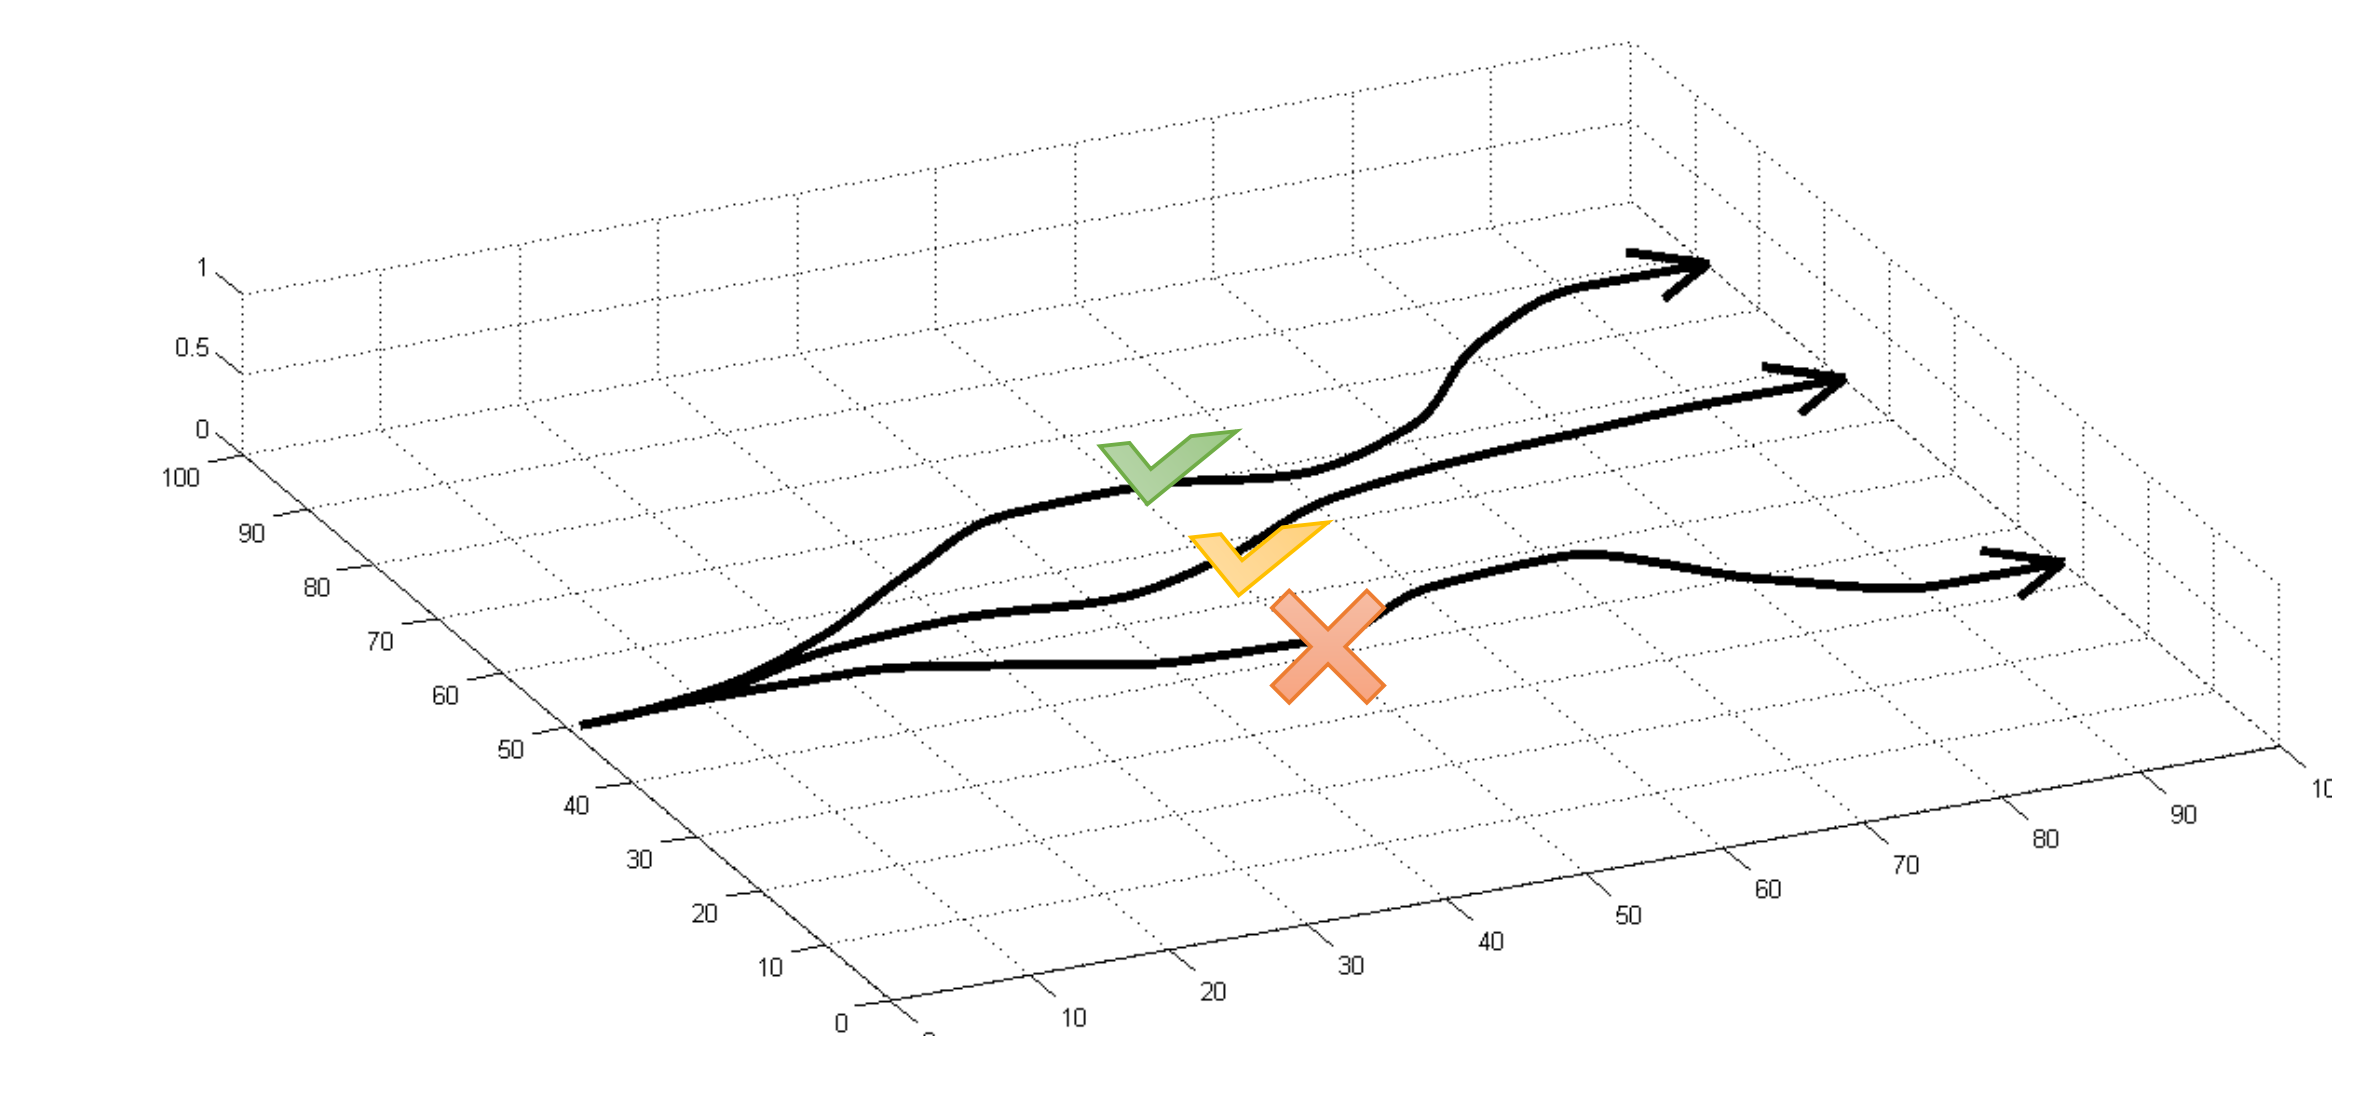
\includegraphics[width=\textwidth,height=0.9\textheight,keepaspectratio]{images/vanilla-policy-gradient/reinforce.png}
    \end{figure}
\end{frame}
